
% !TEX root = /Users/hzd88688126com/Desktop/USFD_Academic-_Report_LaTeX-Template/main.tex
\section{Adaptive Step Size}
\subsection{GASS}
Based on the previous analysis, the step size should be large for fast convergence and getting small to reduce steady state errors. The gradient adaptive step-size (GASS) is implemented with time-varying step $\mu(n)$. The MA(1) process $x(n)=0.9\eta(n-1)+\eta(n)$ with white noise $\eta \sim \mathcal{N}(0, 0.5)$ is simulated. For the GASS, the gradient step will be controlled by a constant $\rho$ and $\psi(n)$. In addition, there are three algorithms which will update the $\psi(n)$. As introduced in guidelines, the Benveniste applies a time-varying adaptive filter, which provides low pass filtering of the instantaneous gradient \cite{mandic2009complex}. Thus, the Benveniste's algorithm is robust to the noise and should be more accurate. The Ang \& Farhang's algorithm replaces the low-pass filter term with a constant $\alpha$. And the Matthews \& Xie's algorithm simplifies the the algorithm by Ang \& Farhang by setting $\alpha$ to zero, which only use the instantaneous gradient to update. Hence, the performance for this algorithm should be relative poor.
\begin{figure}[htbp]
     \centering{}
     \begin{subfigure}[b]{0.4\textwidth}
         \centering
         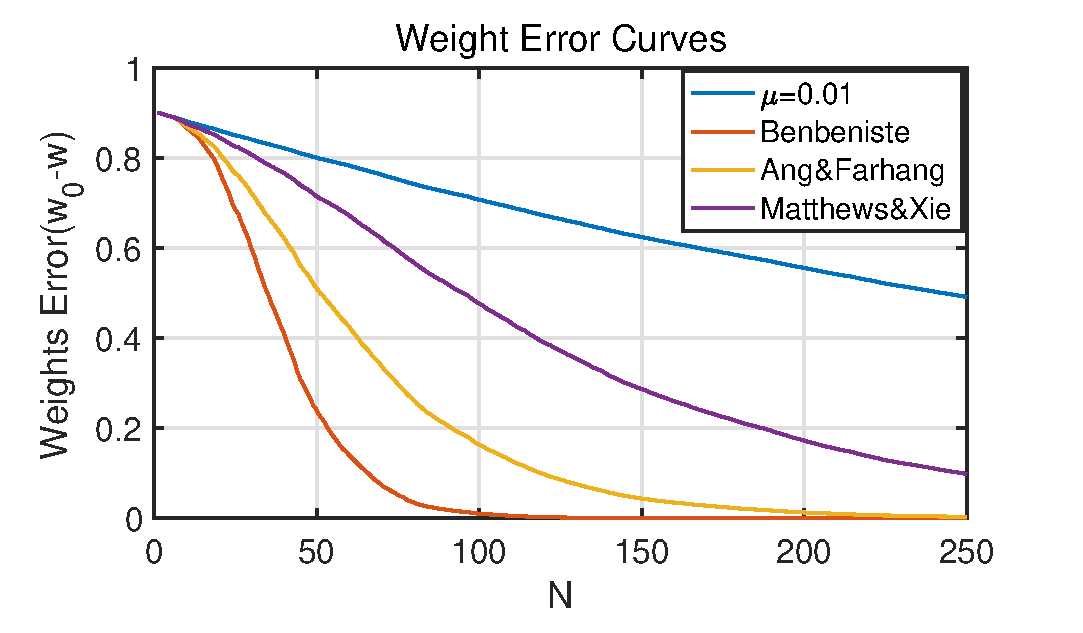
\includegraphics[width=\textwidth]{fig/22/22a1.eps}
     \end{subfigure}
     ~
     \begin{subfigure}[b]{0.4\textwidth}
         \centering
         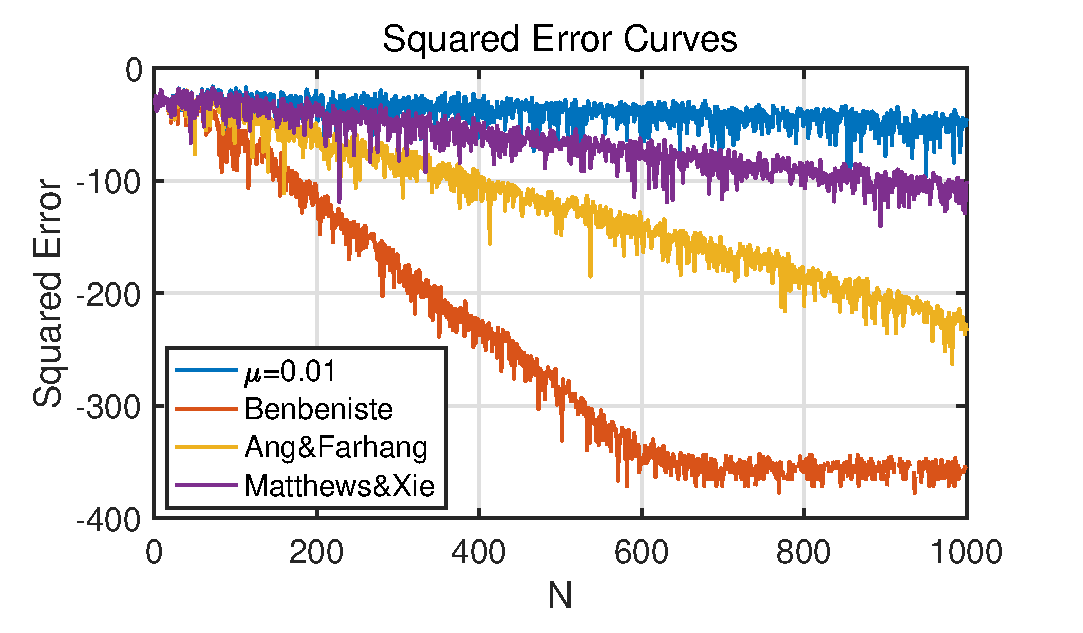
\includegraphics[width=\textwidth]{fig/22/22a2.eps}
     \end{subfigure}
     ~
     \begin{subfigure}[b]{0.4\textwidth}
         \centering
         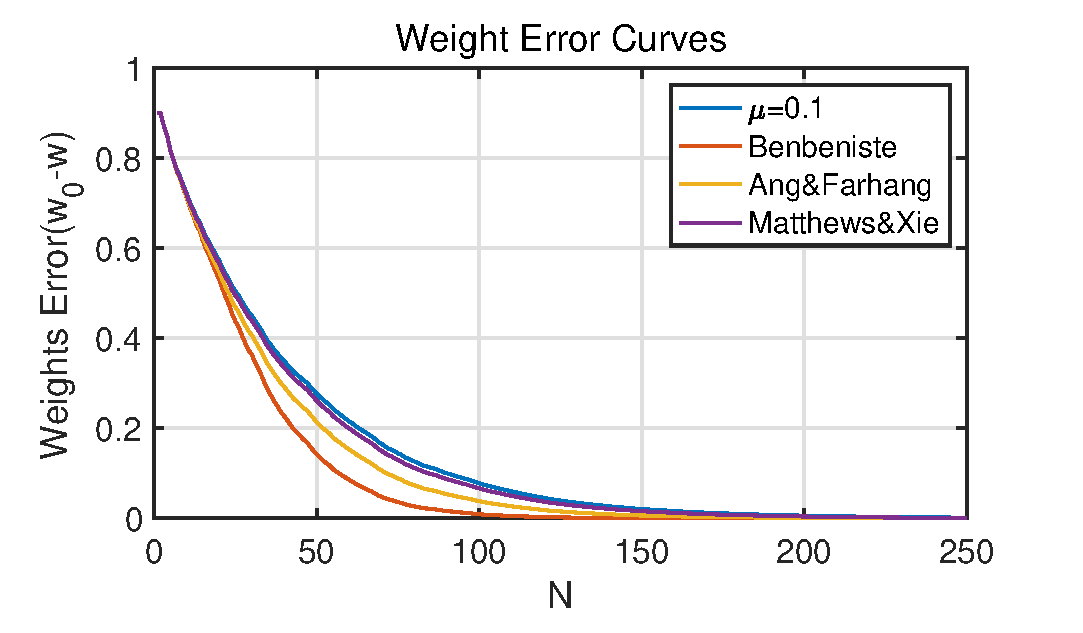
\includegraphics[width=\textwidth]{fig/22/22a3.eps}
     \end{subfigure}
      ~
     \begin{subfigure}[b]{0.4\textwidth}
         \centering
         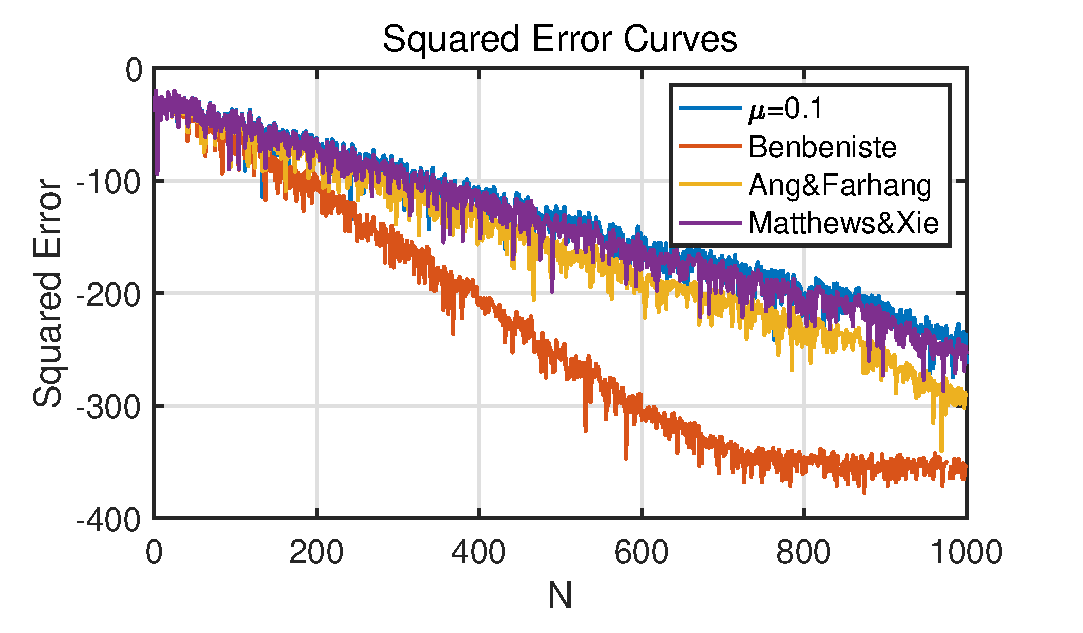
\includegraphics[width=\textwidth]{fig/22/22a4.eps}
     \end{subfigure}
        \caption{GASS estimated weights error and squared error}
        \label{fig:2_2_a}
\end{figure}\\
Fig.\ref{fig:2_2_a} depicts the weight error and learning curves of three algorithms and standard LMS. When setting the initial $\mu$ =0.01, the standard LMS with fixed step has the slowest convergence speed and large steady state error. The Benveniste's algorithm converges before 100 samples, whereas the Ang \& Farhang's converges at 200 samples and Matthews is after 250 samples. However, even if the Matthews's algorithm perform worst among GASS algorithm, it is still slightly better than the standard LMS. When increasing the initial step $\mu=0.1$, all of algorithms converge rapidly with squared error lower than -300$dB$. However, the GASS algorithm requires more computational complexity than the standard LMS.
\subsection{NLMS}
Given a the update weight $\mathbf{w}(n+1)=\mathbf{w}(n)+\mu e_p(n)\mathbf{x}(n)$, the relationship between posteriori error $e_p(n)$ and priori error $e(n)$can be derived by 
\begin{align}
e_p(n)&=d(n)-\mathbf{x}^T(n)\mathbf{w}(n+1)\notag\\
	  &=d(n)-\mathbf{x}^T(n)\mathbf{w}(n)-\mu e_p(n)\mathbf{x}^T(n)\mathbf{x}(n) \notag\\
	  &=e(n)-\mu e_p(n)\|\mathbf{x}(n)\|^2\notag\\
	  &=\frac{e(n)}{1+\mu \|\mathbf{x}(n)\|^2} \label{eq:ep}
\end{align}
Substituting Eq.\ref{eq:ep} into update equation,
\begin{align}
	\mathbf{w}(n+1)&=\mathbf{w}(n)+\mu e_p(n)\mathbf{x}(n)\notag\\
				   &=\mathbf{w}(n)+ \frac{\mu}{1+\mu \|\mathbf{x}(n)\|^2} e(n)\mathbf{x}(n)\notag\\
				   &=\mathbf{w}(n)+ \frac{1}{\frac{1}{\mu}+\|\mathbf{x}(n)\|^2} e(n)\mathbf{x}(n)\notag\\
				   &=\mathbf{w}(n)+ \frac{\beta}{\epsilon+\mathbf{x}^T(n)\mathbf{x}(n) } e(n)\mathbf{x}(n)\label{eq:nllms}
\end{align}
Thus, the update equation based on a posteriori error is equivalent to the NLMS algorithm, where $\epsilon=\frac{1}{\mu}$ and $\beta=1$.
\subsection{GNGD vs GASS}
Based on the NLMS algorithm, the generalized normalized gradient descent (GNGD) applies a time-varying $\epsilon(n)$. Compared with the Benveniste's algorithm, the GNGD algorithm converges rapidly of weight estimation approximately at 40 samples when the initial step $\mu=0.1$. The squared error
for the GNGD is smaller as well. However, when increasing the initial step $\mu=1$, the Benveniste's algorithm converges faster than the GNGD. Thus, the performance of the GASS algorithm is significantly affected by initial step $\mu$, while it is not a problem for the GNGD algorithm.
\begin{figure}[htbp]
     \centering
     \begin{subfigure}[b]{0.4\textwidth}
         \centering
         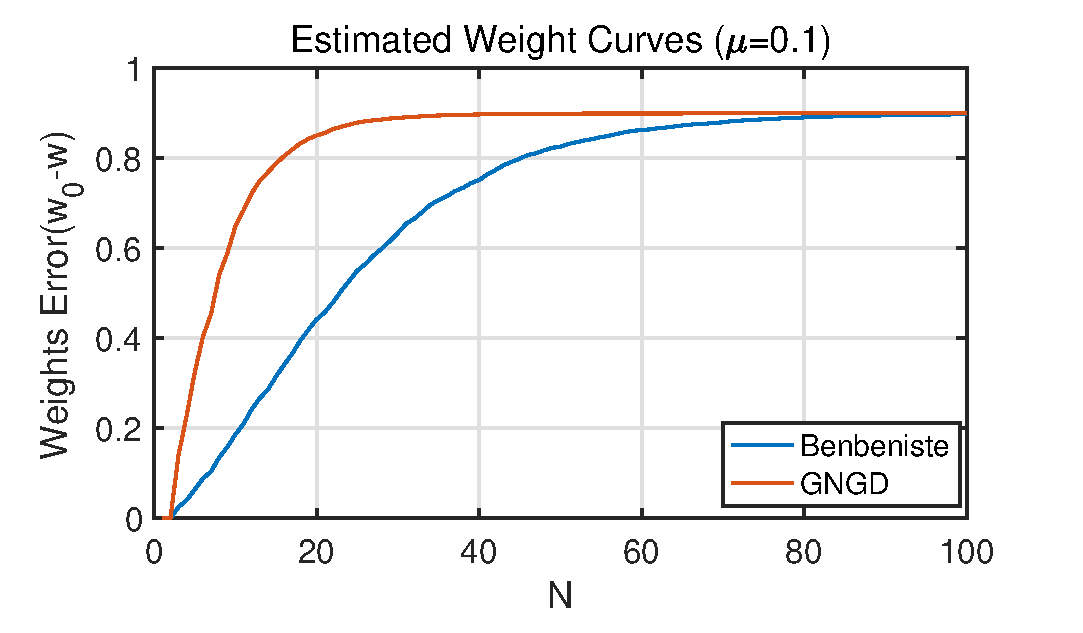
\includegraphics[width=\textwidth]{fig/22/22c1.eps}
     \end{subfigure}
     ~
     \begin{subfigure}[b]{0.4\textwidth}
         \centering
         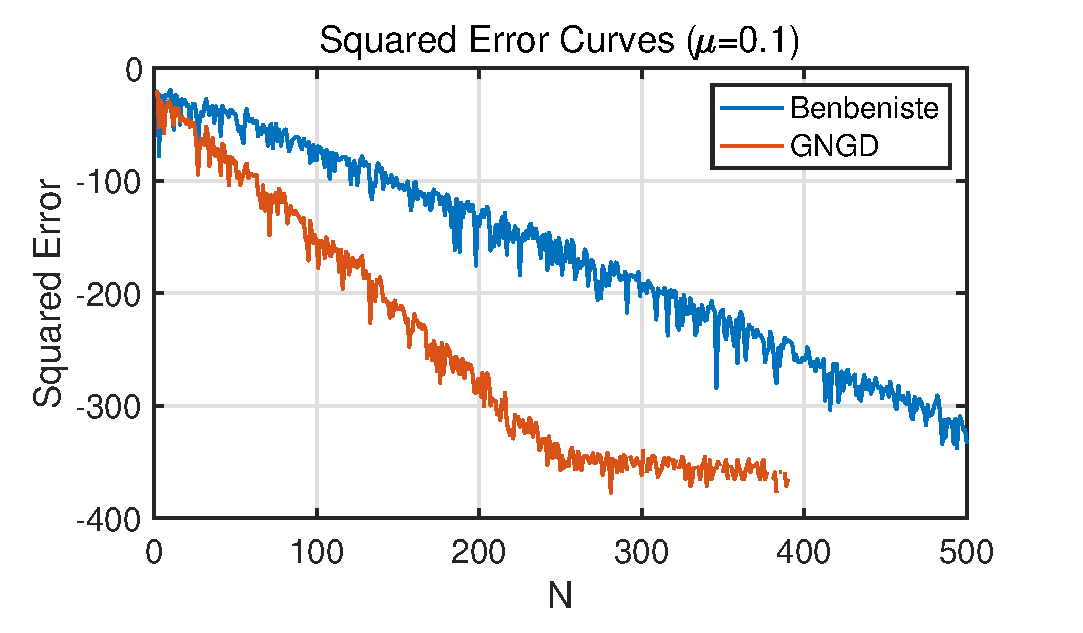
\includegraphics[width=\textwidth]{fig/22/22c2.eps}
     \end{subfigure}
     ~   
      \begin{subfigure}[b]{0.4\textwidth}
         \centering
         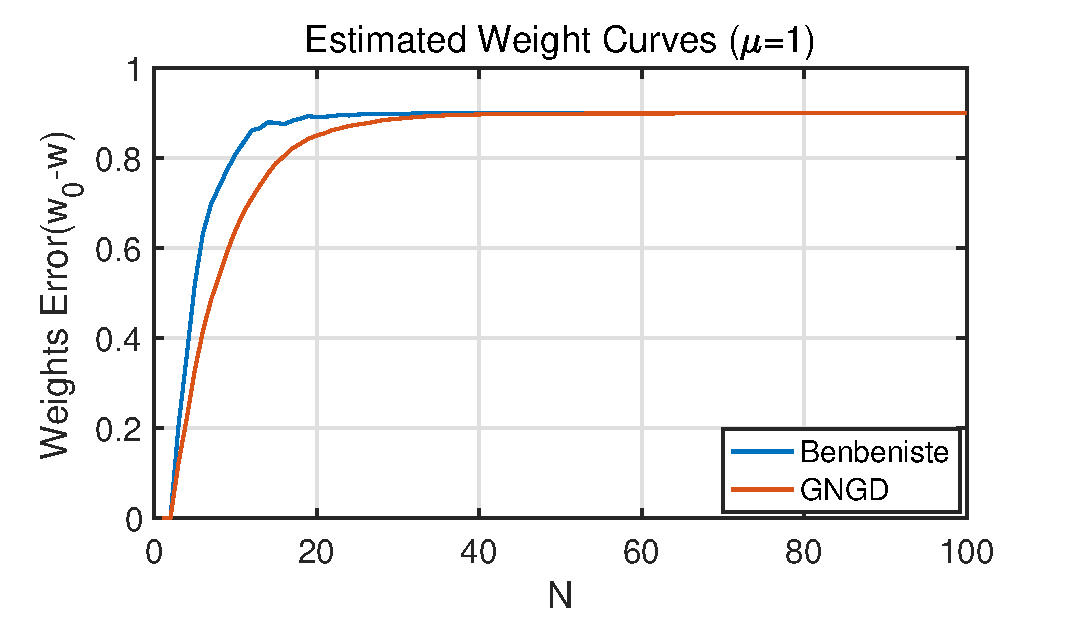
\includegraphics[width=\textwidth]{fig/22/22c3.eps}
     \end{subfigure}
     ~
     \begin{subfigure}[b]{0.4\textwidth}
         \centering
         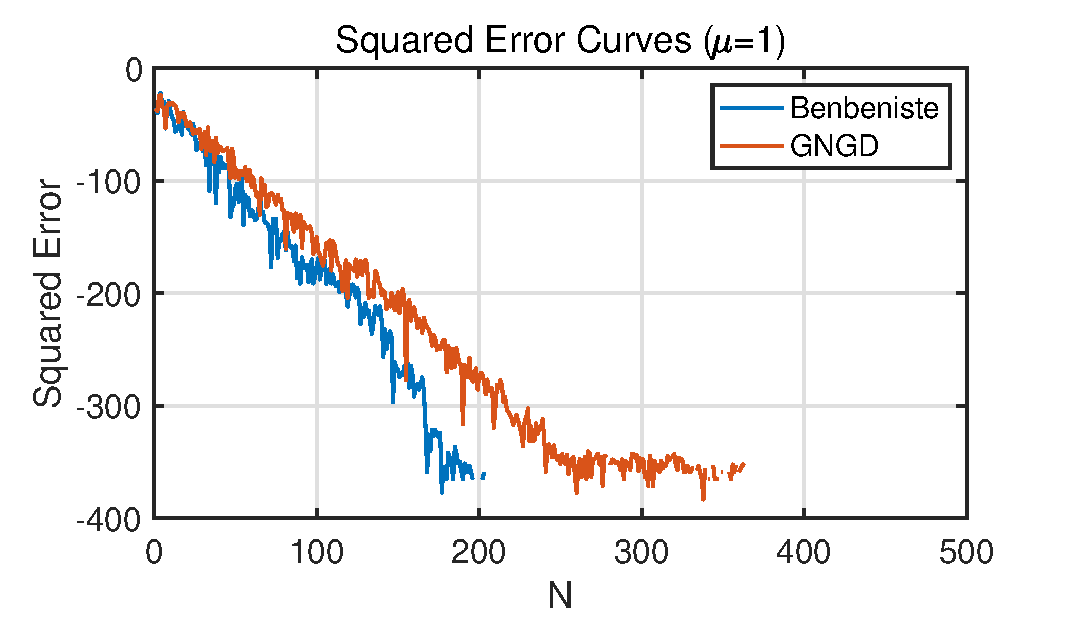
\includegraphics[width=\textwidth]{fig/22/22c4.eps}
     \end{subfigure}
        \caption{GAGN and Benveniste's GASS estimated weights and squared error}
        \label{fig:2_2_c}
\end{figure}\\
As to the complexity of these two algorithms, the computation complexity is caused by the matrix product in step update process. The Benveniste's algorithm, as shown below,
\begin{equation}
	\mathbf{\psi}(n)=[\mathbf I\overbrace{-\underbrace{\mu(n-1)\mathbf x(n-1)\mathbf {x}^T(n-1)}_{N^2}]\mathbf{\psi}(n-1)+}^{2N}\underbrace{e(n-1)\mathbf x(n-1)}_{N}
\end{equation}
has $O(N^2)$ multiplications, if the model order is $N$. The reason is that the Benveniste's algorithm applies matrix outer production which introduces a matrix result. Therefore, the computational complexity of the Benveniste grows quadratically. For the GNGD, as shown below,
\begin{equation}
	\epsilon(n+1)=\epsilon{n}-\rho\mu\frac{e(n)e(n-1)\overbrace{\mathbf x^T(n)\mathbf x(n-1)}^{N}}{(\epsilon(n-1)+\underbrace{\|\mathbf x(n-1)\|^2}_{N})^2}
\end{equation}
It only has inner product of $\mathbf x(n)$, resulting in a numerical value. Hence, the computational complexity is reduced over order $M$ which is $O(N)$.







